\chapter{Timing en optimalizatie}
\label{timing-optimization}
Voor een correcte werking van het geheugen, is het van belang dat de verschillende controlesignalen in een bepaalde volgorde verwerkt en doorgegeven worden.
Bovendien is er ruimte voor optimalisatie door al de signalen even snel te maken als het critisch pad. In het eerste deel van dit hoofdstuk zal de invloed van architecture en sizing onderzocht worden op de timing van de signalen. De constraints en vrijheidsgraden die hier uit volgen zullen dan gebruikt worden in het tweede deel van dit hoofdstuk om een optimale architecture te vinden.

\section{Timing}
Het ontwerp van dit geheugen gaat tot het niveau van het globalblock \ref{globalblock}, hierbij wordt de veronderstelling gemaakt dat alle signalen tegelijkertijd binnen komem in het globelblock. Hierna propageren de signalen door logica tot ze verschillende transistoren rond de BL aansturen. De aansturing van deze transistoren omvatten de eerste critische timing constraints. Vervolgens worden de muxen en SA aangesloten, deze zullen de tweede timing constraints bevatten.

\subsection{Critische timing voor het (de)selecteren cell}
\paragraph{}
Timings problemen rond het (de)selecteren van de cell komen door het een verschill in timing voor het (de)selecteren van de load en cell. Indien de load geselecteerd wordt voor de cell zal de bitline vroegtijdig beginnen opladen naar de voedingspanning. Wanneer de cell dan geselecteert is zal de bitline naar een betekenis volle spanning getrokken worden. Afhankelijk van het tijds verschill tussen deze twee evenementen, zal de bitlijn terug omlaag getrokken worden, wat resulteert in een energie verspilling. Dit wordt geillustreerd in figuur \ref{fig:critisch_timing1}. Indien de cell gedeselecteert wordt voordat de load gedeselecteerd is, Zal de bitline ook opladen naar de voedingspanning. Dit heeft als gevolg dat het ontladen van de bitlijn langer zal duren en de overbodige oplading resulteert ook in een energie verspilling. Door de keuze van logica (zie figure TODO) zal afhankelijk van het tijds verschill, de mux te vroeg worden afgeschakelt. Waardoor de knoop achter de mux niet volledig ontladen zal zijn. Dit heeft geen nadelige gevolgen door dat de capaciteit op dit knooppunt heel klein is en er bijgevolge een verwaarloosbare ladings injectie is in de volgende lees cyclus. Al dit word geillustreert in figure \ref{fig:critisch_timing2}.  


\begin{figure}[h!]
\centering
\subfloat[]{ 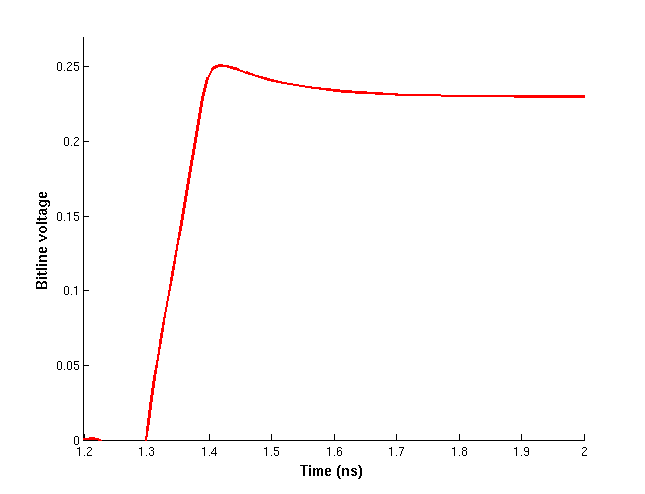
\includegraphics[width=0.5\textwidth] {../fig/hfdstk-timing-crit1.png} \label{fig:critisch_timing1}}
\subfloat[]{ 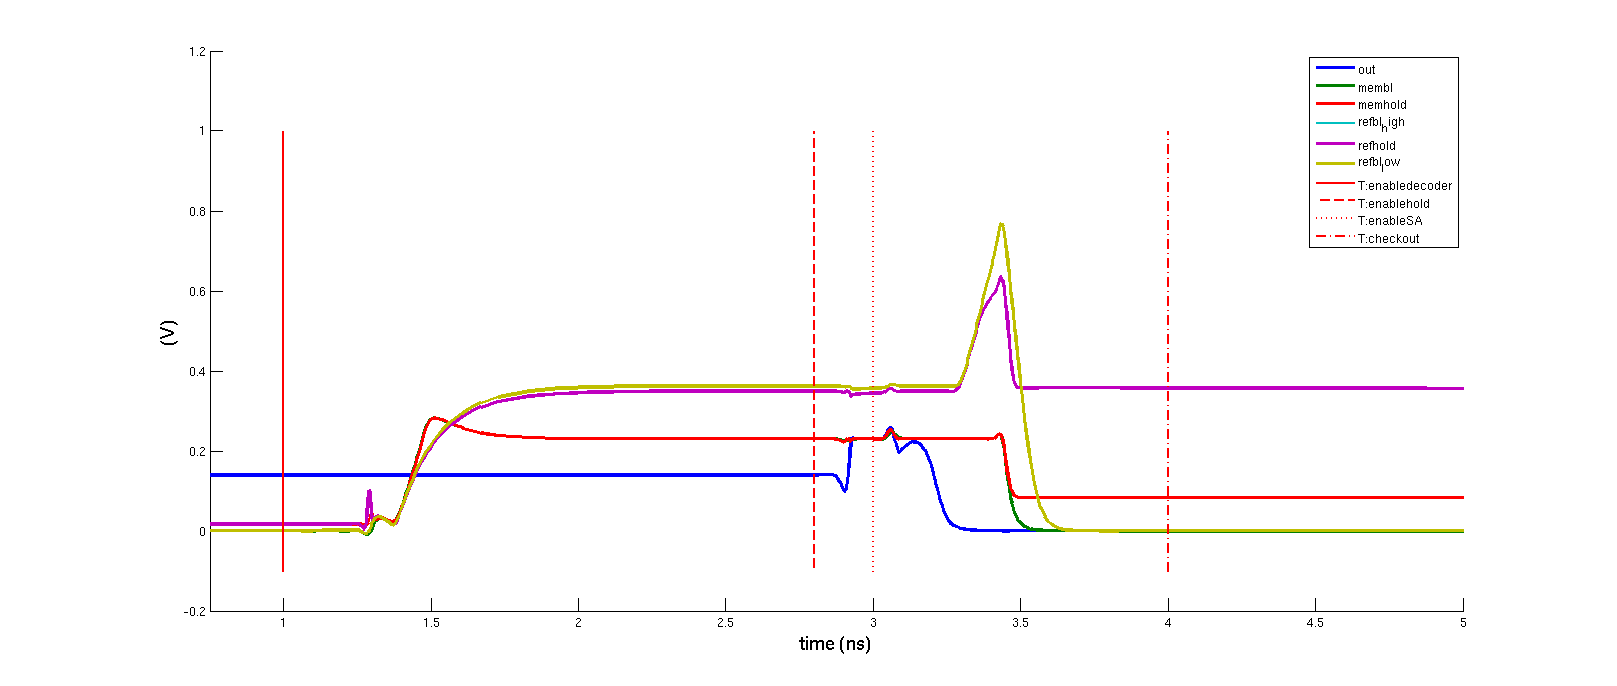
\includegraphics[width=0.5\textwidth] {../fig/hfdstk-timing-crit2.png} \label{fig:critisch_timing2}}
\caption{Timing problemen bij de bitlijn}
\end{figure}

\paragraph{}
De timing begint in het globalblock. Het circuit en timings diagram word geillustreerd in figuren \ref{fig:gb_timing1} en \ref{fig:gb_timing2}. T1 en T2 stellen het moment voor dat de signalen uit de Bitlijn en Woordlijn decoder komen. T3 stelt het moment voor dat het signaal uit de referentie buffer komt. T1 en T3 zou op het zelfde moment moeten aankomen om een optimale timing te hebben. Indien dit niet het geval is zal de referentie bitlijnen al aanstaan vooralleer de cell bitlijn aan komt te staan. Indien er een groot aantal referentie bitlijnen zijn zal dit resulteren in een grote energie verspilling. Om deze timing te verwezelijken zijn er twee opties. De eerste is het kiezen van een kleine bitlijn decoder en een grote woordlijn decoder. Dit zal voor een kleine T1 zorgen door een kleine delay in de bitlijn decoder. Dit zal een grotere T3 geven door dat de referentie buffer meer capaciteit heeft om op te laden. Een evenwicht kan zo gevonden worden om T1 en T3 op het zelfde moment te doen verschijnen. Deze eerste optie beperkt de mogelijke architecture intensief en zal timings constraints voor T2 teniet doen zoals later zal blijken. De tweede optie voor het matchen van T1 en T3 is het vertragen van T3. Een vertraging kan gerealiseert worden door het invoeren van delay elementen of door het verslechteren van de buffer. In practijk is ondervonden dat het invoeren van vertragings element meestal een te grote delay introduceert. Vandaar dat in de final design een buffer werdt gemaakt die niet optimaal is naar snelheid. Om het energie verbruik van de referentie bitlijnen verder te verminderen werden niet al de bitlijnen in de array gebruikt voor het generen van het referentie signaal.

\begin{figure}[!ht]
  \centering
  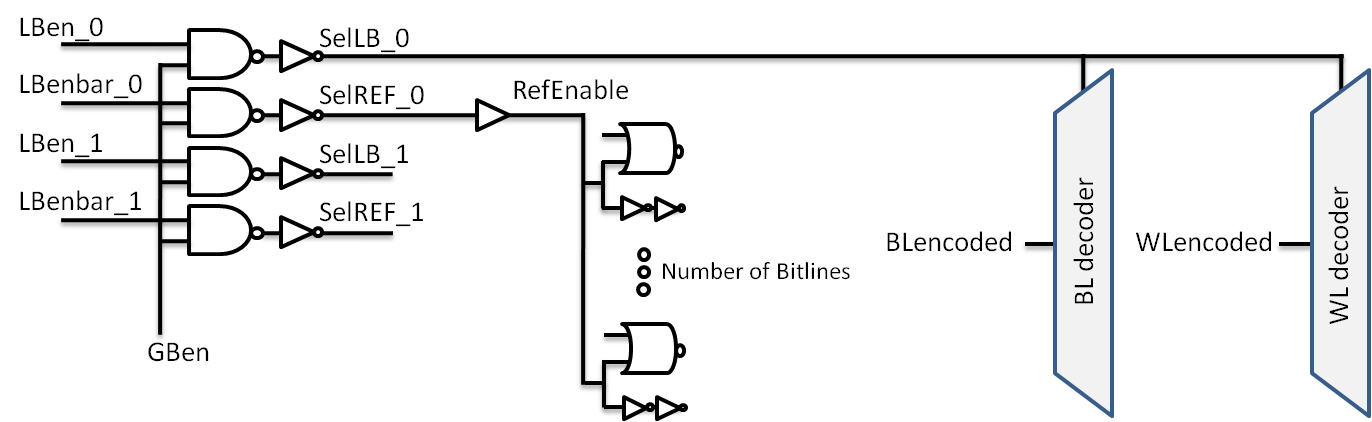
\includegraphics[scale=0.6]{../fig/hfdstk-timing-gb1.png}
  \caption{Globalblock logica}
  \label{fig:gb_timing1}
\end{figure}

\begin{figure}[!ht]
  \centering
  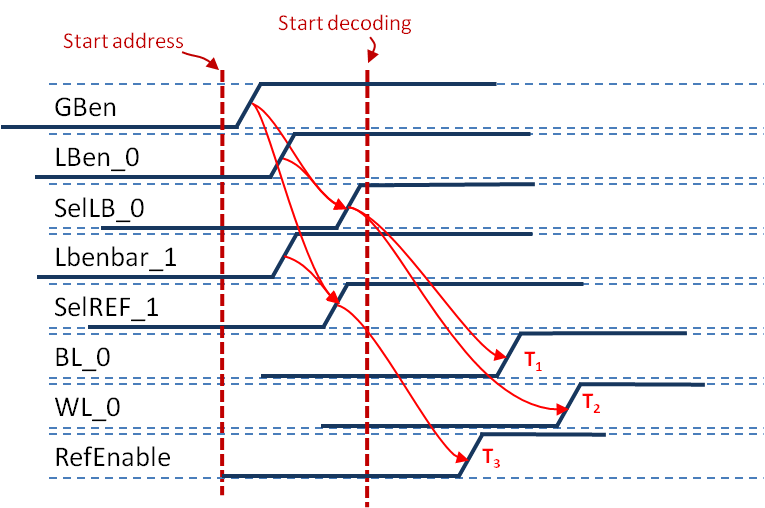
\includegraphics[scale=0.9]{../fig/hfdstk-timing-gb2.png}
  \caption{Timing globalblock}
  \label{fig:gb_timing2}
\end{figure}

\paragraph{}
Eens de sigalen uit de decoders komen worden deze gevoed in de controle logica voor de memory array. Het circuit en timing diagram is geillustreerd in figuren \ref{fig:lbcell_timing1} en \ref{fig:lbcell_timing2}. Bij het aanschakelen van de cell zouden de cell vroeger of tegelijk als de last moeten geschakelt worden. Op het timings diagram wordt dit geillustreert als T4 = T5 = T6. Door de implementatie van de logica is dit niet mogelijk aangezien er altijd een inverter vertraging verschil is tussen T4 en T5. Deze vertraging is minimaal en kan getollereerd worden door dat de bitlijn in elk geval moet op geladen worden tot minimum $V_{LRS}$. Bij lage voedingspanningen komt dit probleem daarentegen terug boven. T6 wordt bepaalt door woordlijn decoder en woordlijn buffers. Deze vertraging zou zo gemaakt moeten worden dat deze vroeger of gelijk met T5 valt. Bij het afschakelijke van de cell zijn de omgekeerde voorwaarden nodig namelijk, De last zou vroeger of gelijk als de cell moeten afgeschakelt moeten worden. Deze voorwaarde is voldaan als T7 voor T8 en T9 komt. Door de inverter is T7 altijd voor T8, T9 daarentegen word bepaalt door de woordlijn decoder en buffer en zou voor T7 moeten komen. \\
De timing van de controle logica voor de memory array staat in het circuit vast op de timing van de woordlijn na. Deze moet moet geselecteerd worden voor de sourcelijn geselecteerd is en moet gedeselecteerd worden na dat de last gedeselecteerd is. De timing van de woordlijn wordt expliciet bepaalt door de grote van de woordlijn decoder en impliciet door de grote van de bitlijn decoder dat de grote van de woordlijn buffer bepaalt. Figure \ref{fig:decoder_dep} geeft de delay van verschillende grotes van woorlijn decoders + buffer ifv verschillende grotes van bitlijn decoders weers ... TODO

\begin{figure}[!ht]
  \centering
  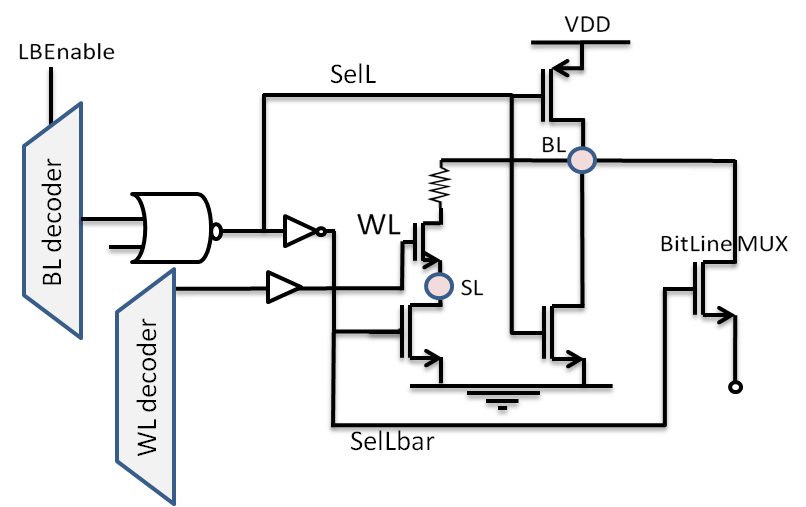
\includegraphics[scale=0.6]{../fig/hfdstk-timing-lbcell1.png}
  \caption{Controle logica memory array}
  \label{fig:lbcell_timing1}
\end{figure}

\begin{figure}[!ht]
  \centering
  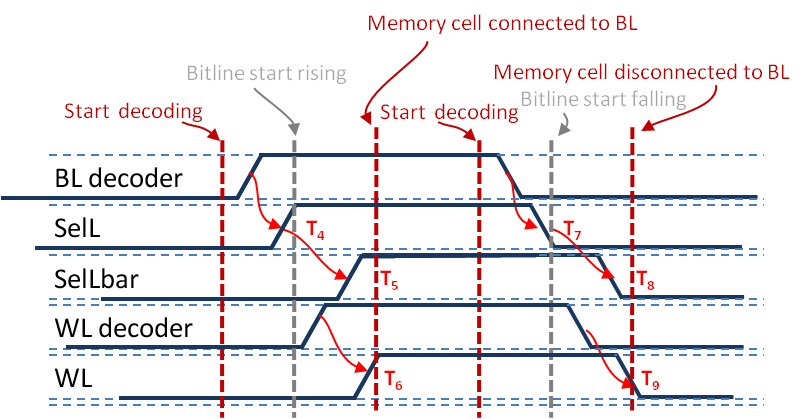
\includegraphics[scale=0.9]{../fig/hfdstk-timing-lbcell2.png}
  \caption{Timing controle logica memory array}
  \label{fig:lbcell_timing2}
\end{figure}

\begin{figure}[!ht]
  \centering
  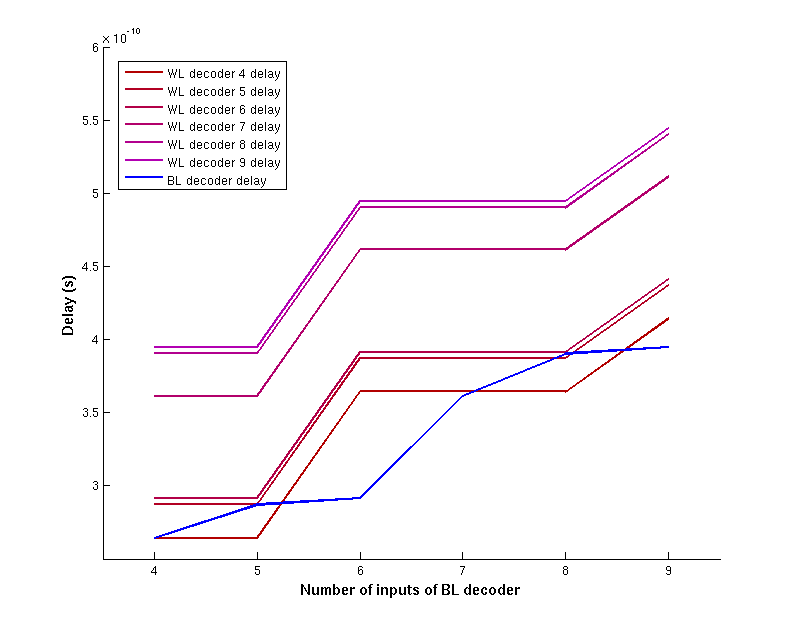
\includegraphics[scale=0.6]{../fig/hfdstk-timing-decoder-dep.png}
  \caption{Delay van woordlijn decoders + buffers ifv bitlijn decoders}
  \label{fig:decoder_dep}
\end{figure}

\paragraph{}
De timings voorwaarden voor het selecteren en deselecteren van de referentie cell, zijn het zelfde als die van de memory cellen. Het circuit en timing diagram is geillustreerd in figuren \ref{fig:lbref_timing1} en \ref{fig:lbref_timing2}. Anders als bij de memory cellen worden de timings voorwaarden al in de logica zelf voldaan door dat de woorlijnen worden aangestuurd door een signaal dat rechtstreeks van de bitlijn decoder komt. Dit signaal word dan vertraagt door twee invertoren om de juiste timing te verwezelijken.


\begin{figure}[!ht]
  \centering
  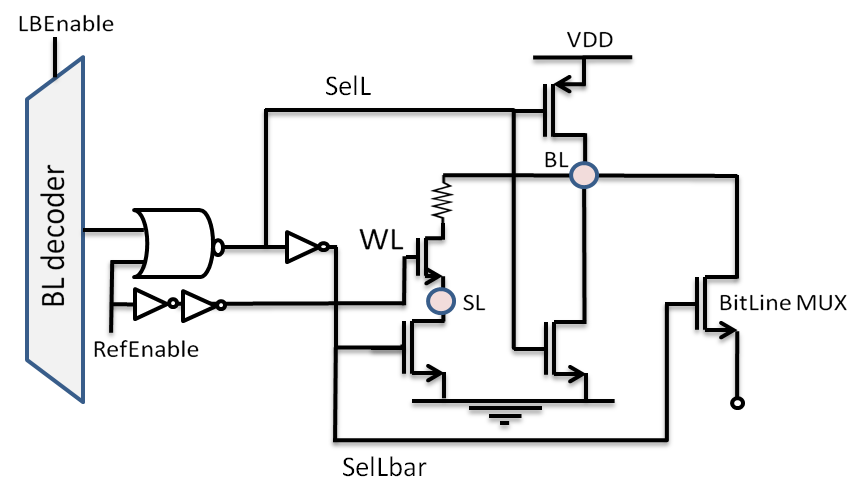
\includegraphics[scale=0.6]{../fig/hfdstk-timing-lbref1.png}
  \caption{Controle logica memory array}
  \label{fig:lbref_timing1}
\end{figure}

\begin{figure}[!ht]
  \centering
  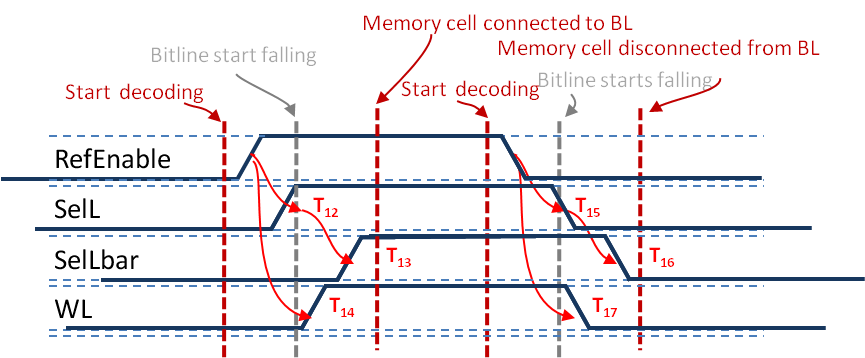
\includegraphics[scale=0.9]{../fig/hfdstk-timing-lbref2.png}
  \caption{Timing controle logica memory array}
  \label{fig:lbref_timing2}
\end{figure}

\subsection{Critische timing voor het uitlezen van de cell}
Eens de cell geselecteerd is wordt de bitlijn opgeladen. De volgende stap is dit signaal voeden aan de sense amplifier. Dit signaal wordt eerst door een eerst mux geleid om uit de localblock te geraken. Vervolgens word het signaal door een tweede mux geleidt die als sample en hold dient voor de sense amplifier. Figuren \ref{fig:sa_timing1} en \ref{fig:sa_timing2} illustreren het circuit en timing rond de sense amplifier. Eens de bitlijn is aangesloten wordt de eerste mux automatisch aangesloten zoals uitgelegd in de vorige paragraven. T19 stelt het tijdsstip voor waar de tweede mux aangesloten moet worden. Deze timing is niet crutiaal, de mux mag zowel aangesloten worden voor als na het aansluiten van de bitlijn mux. Het tijdstip van afsluiten van deze mux (T22) is daarentegen wel belangrijk. Dit moet namelijk gebeuren voor de bitlijn mux afgesloten is (T21) anders zullen er 2 charge injections voorkomen ipv een. Om een zo snel mogelijke latching van de sense amplifiers te hebben, is het tijd stip waar de sense amplifier (T20) aangesloten word belangrijk. Wanneer de sense amplifier juist word aangesloten treed er een latching effect plaats waar de sense amplifier zich gedraagd als of er geen last aan hangt dit effect werd beschreven in sectie \ref{TODO}. Eens dit voorbij is zal de sense amplifier latchen aan de snelheid van de RC constante van de bitlijn. Om een snelle latching te hebben moet de tweede mux afgesloten worden voor dit latching effect voorbij is.
Tenslotte kan de sense amplifier afgesloten worden eens het latchen voorbij is.

\begin{figure}[!ht]
  \centering
  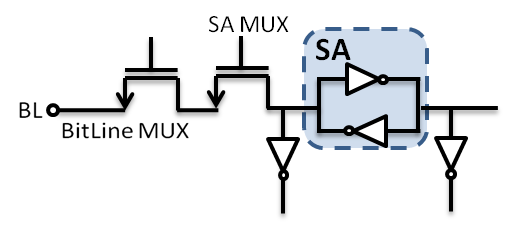
\includegraphics[scale=0.6]{../fig/hfdstk-timing-sa1.png}
  \caption{logica rond SA}
  \label{fig:sa_timing1}
\end{figure}

\begin{figure}[!ht]
  \centering
  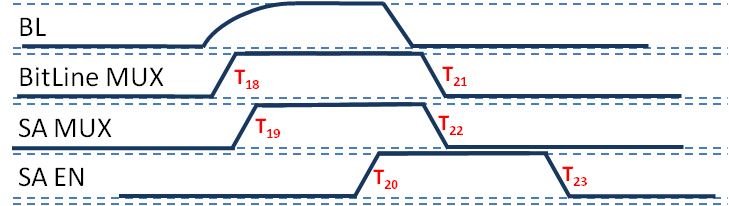
\includegraphics[scale=0.9]{../fig/hfdstk-timing-sa2.png}
  \caption{Timing logica rond SA}
  \label{fig:sa_timing2}
\end{figure}

\section{Analyse verschillende geheugenconfiguraties}
\paragraph{}
Het finale geheugen zal 4 Mbit groot zijn. Heel wat configuraties zijn mogelijk om deze grote te verwezelijken. Om deze mogelijkheden wat in te perken worden de volgende beperking op gelegt. Het aantal Woordlijnen moet groter of gelijk zijn aan het aantal bitlijnen. Hierdoor zal Het ontladen van de bitlijn sneller verlopen. Dit levert 20 mogelijke configuraties voor aantal bitlijnen,woordlijnen en globalblocks. Deze configuraties worden vergeleken op basis van hun oppervlakte, energie verbruik en leessnelheid. 

\subsection{Evaluatie criteria voor de geheugenconfiguraties}
Het Oppervlakte wordt berekend op basis van de lengtes en breetes van de transistoren. Gardrings en verbindings lijnen worden niet meegerekend in de berekeningen van het oppervlakte van de logica. De lengte van de geheugen cellen wordt 1.5*6F genomen en voor de breete wordt 2*6F genomen \cite{ppt:cosemans}. Hoewel deze afmetingen voor een MTJ geheugen cell zijn, geven ze een goedde schatting van het oppervlakte van een Memristor geheugencell. Verder is in dit oppervlakte de grote van bitlijn, woordlijn en selectlijn meegerekend. \\
Het energie verbruik word berekend door de stroom van de voedingspanning te integreren over de tijd en te vermenigvuldigen met de voedingspanning. De signalen die binnen komen in een global block, komen van ideale spice bronnen. Dit geeft als gevolg dat er een charge injectie is naar de voedingspanning (zie bijlage \ref{app:chargeinj}). Dit heeft een invloed op de energie berekeningen maar er worden geen pogingen gedaan op deze te corrigeren. Verder wordt het aantal referentie cellen ook constant gehouden voor de verschillende configuraties. Dit wordt gedaan om het energie verbruik te verkleinen en omdat men maar een beperkt aantal cellen nodig heeft om een goede referentie te krijgen.\\
De leessnelheid is afhankelijk van de verschillende controle signalen in de lees cyclus en deze gebeurd als volgt. De lees cyclus begint wanneer de signalen binnen komen in de globalblock. De SA wordt aangesloten wanneer het verschil tussen de memory bitlijn en de referentie bitlijn 100mV bedraagd. Hierdoor wordt het tijds verschil tussen geheugens met een klein aantal woordlijnen en geheugens met een groot aantal woordlijnen verkleind, wat een betere concurentie geeft. In het finale geheugen ontwerp zal de leessnelheid verder opgedreven worden door deze 100mV voltage verschil te verkleinen. Verder word er ook altijd een cell met een HRS uitgelezen aangezien deze de bitlijn langer moet opladen om tot aan de 100mV verschil te komen wat een realistischere leessnelheid geeft. De lees cyclus eindigd wanneer het bitlijn voltage terug naar de grond is getrokken. Figure \ref{fig:leescyclus} illustreed de hele leescyclus.

\begin{figure}[!ht]
  \centering
  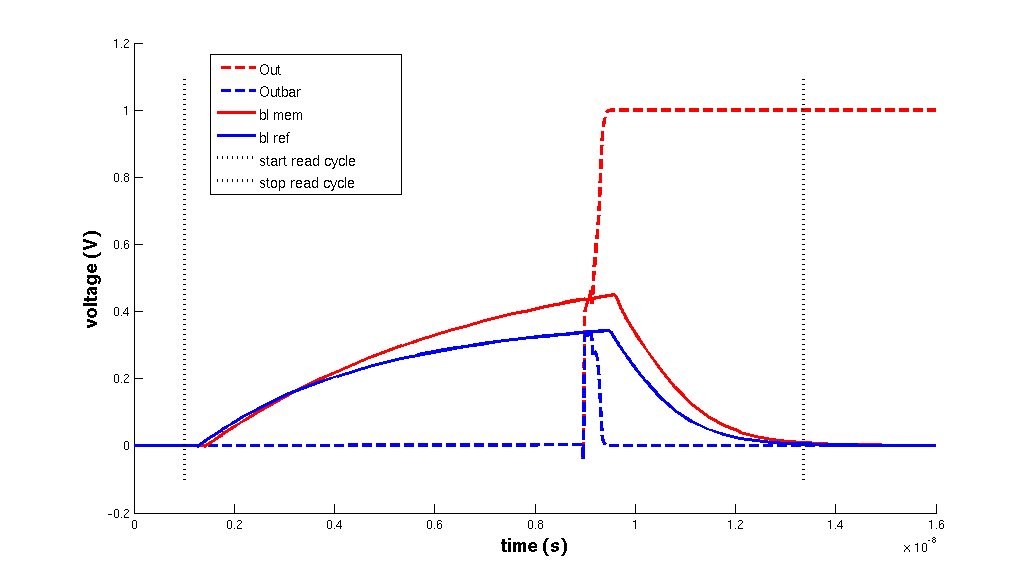
\includegraphics[scale=0.6]{../fig/hfdstk-timing-leescyclus.png}
  \caption{Timing controle logica memory array}
  \label{fig:leescyclus}
\end{figure} 

\subsection{Vergelijking van de geheugenconfiguraties}
Er werden 20 mogelijke geheugenconfiguraties geselecteert als kandidaat voor het finale ontwerp, hun positie in de evaluatie ruimte wordt getoont in figuur \ref{fig:final20all1}. Hierop staat het energie verbruik op de x-as, de delay op de y-as en het oppervlakte gebruik wordt geindiceert door de grote van de punten. Het energie verbruik en delay wordt voornamelijk bepaalt door het aantal woordlijnen en bitlijnen. De delay wordt voornamelijk bepaalt door het opladen van de bitlijnen, wat dan ook de voornamste vorm van energie verbruik is. De snelheid van de bitlijnen wordt dan weer bepaalt door het aantal woordlijnen wat gezien kan worden in figuur \ref{fig:final20all2}. Het aantal bitlijnen beinvloed dan weer meer het energie verbruik. Dit extra energie verbruik gaat teneerste naar de woorlijn buffers, tentweede naar de bitlijn decoders en tenslotte naar de bitlijn zelf. Deze laatste is door dat de bitlijn bij het deselecteren van de cell langer aanblijft dan bij een kleiner aantal bitlijnen. Dit is ook de reden waarom een groter aantal bitlijnen een langere delay heeft. Bij alle geheugen configuraties gaat het vermogen verbruik eerst naar de geheugecell, vervolgens naar de logica, vervolgens naar de buffers en ten slotte naar de sense amplifiers. Het oppervlakte wordt bepaalt door het aantal globalblocks en de grote van de decoders. Een groot aantal woordlijnen in combinatie met een klein aantal bitlijnen geeft de noodzaak aan een groot aantal globalblocks en dit geeft een groot oppervlak als gevolg.\\
Als conclusie kan gezegt worden dat de optimale geheugen configuratie bestaat uit een klein gelijk aantal woordlijn en bitlijnen wat een optimum zal geven voor energie verbruik en delay, en een sub optimum zal geven voor oppervlakte.

\begin{figure}[h!]
  \centering
  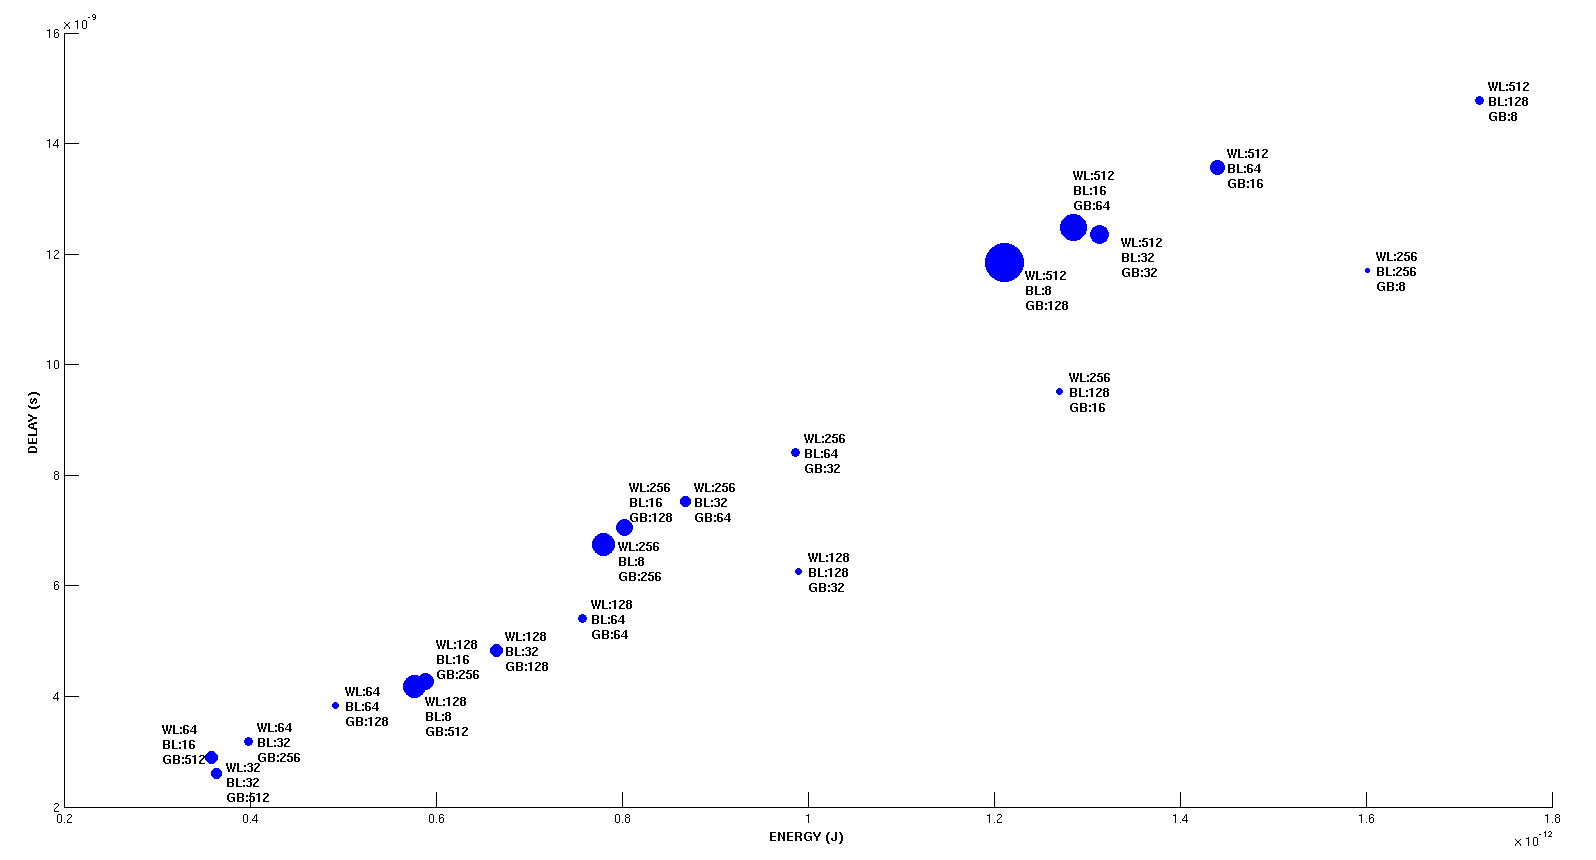
\includegraphics[scale=0.5, angle = 90]{../fig/hfdstk-timing-all-sol1.png}
  \caption{Timing controle logica memory array}
  \label{fig:final20all1}
\end{figure} 

\begin{figure}[h!]
  \centering
  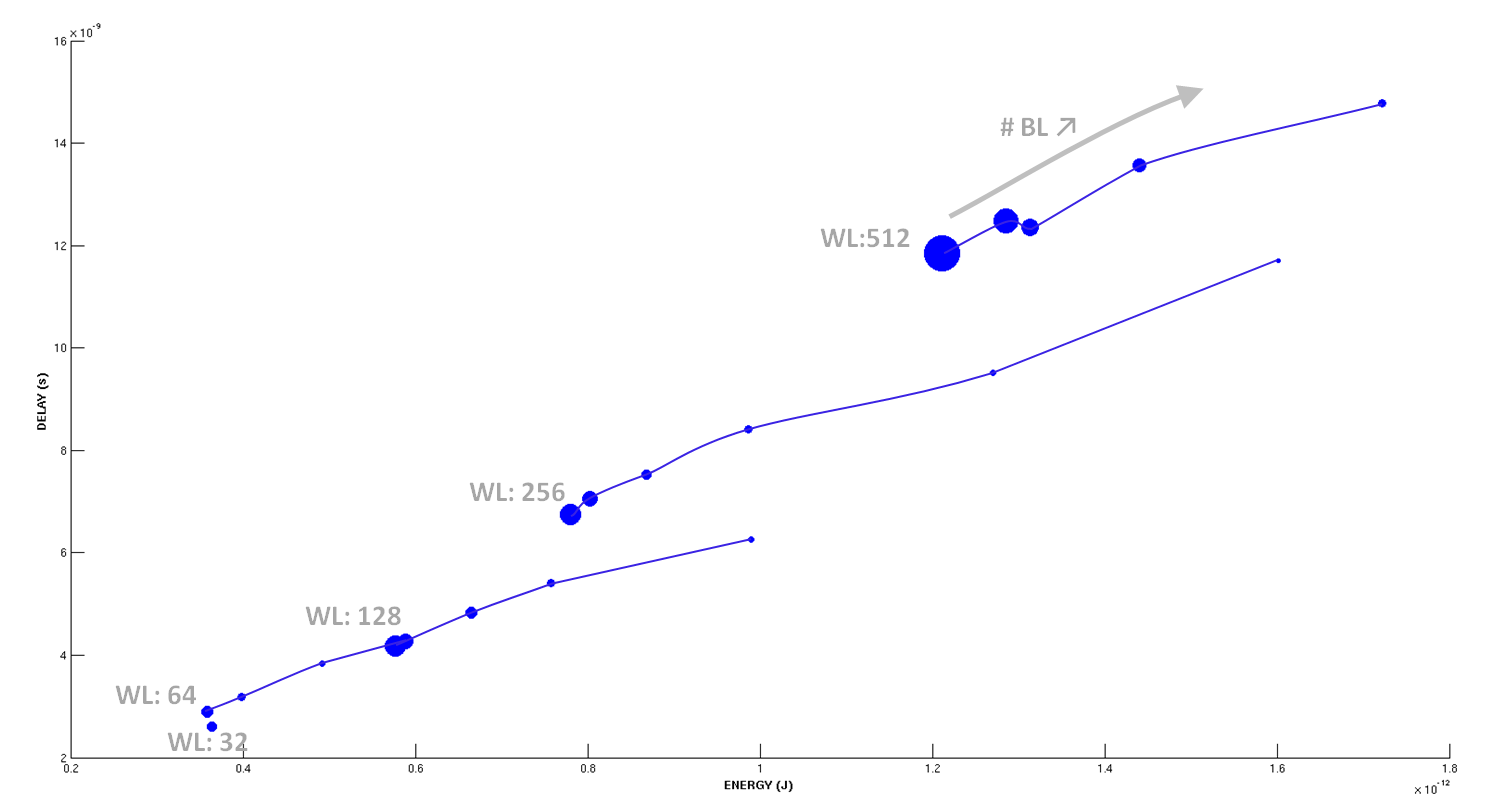
\includegraphics[scale=0.6]{../fig/hfdstk-timing-all-sol2.png}
  \caption{Timing controle logica memory array}
  \label{fig:final20all2}
\end{figure} 
